\chapter{Observation and data reduction}\label{chap:data}
\thispagestyle{fancy}

\section{VLT/MUSE}

NGC 6397 was observed with the Multi Unit Spectroscopic Explorer (MUSE) at the Very Large Telescope (VLT) of the European Southern Observatory (ESO) at Paranal, Chile. MUSE is an integral field spectrograph (IFS). MUSE works by separating the full field of view ($1' \times 1'$) into 24 sub-fields ($2.5" \times 60"$). Each of these 24 is them process by 24 identical but independent integral field units (IFU). Each IFU consists of an image slicer, an spectrograph and a CCD. Each IFU illuminates a $4 \text k \times 4 \text k$ CCD after slicing the light into 48 slit-like slices (with size $\sim 15" \times 0".2$), and decomposing it via a volume phase holographic grating \citep{barden_volume-phase_1998}. The grating achieves a spectral resolution of 1750 at 4650 Å to 3750 at 9300 Å. The data from the 1152 slices is then reconstructed into a $1' \times 1'$ datacube (two spatial and one wavelength axis) with a $0".2$ spatial resolution covering from 4750 Å to 9350 Å sampled at 1.25 Å \citep{bacon_muse_2010}. 

NGC 6397 was observed during the third commissioning period  (ESO Programme ID 60.A-9100(C) \cite{bacon_muse_2014}). The observation were taking from July 26nd to August 3rd, 2014. The observations covered the central part of NGC 6397 ($\sim 3'.5$ from the cluster center see fig~\ref{fig:clustermuse}). The dataset consists of 23 different pointings of MUSE with short exposure times ranging from 25-60 seconds. In total they obtained 127 exposures of the 23 different $1' \times 1'$ regions (see fig~\ref{fig:clustermuse}). This gives a total integration time of 95 minutes for all the observed part of the cluster.


\begin{figure}[H]
        \centering
        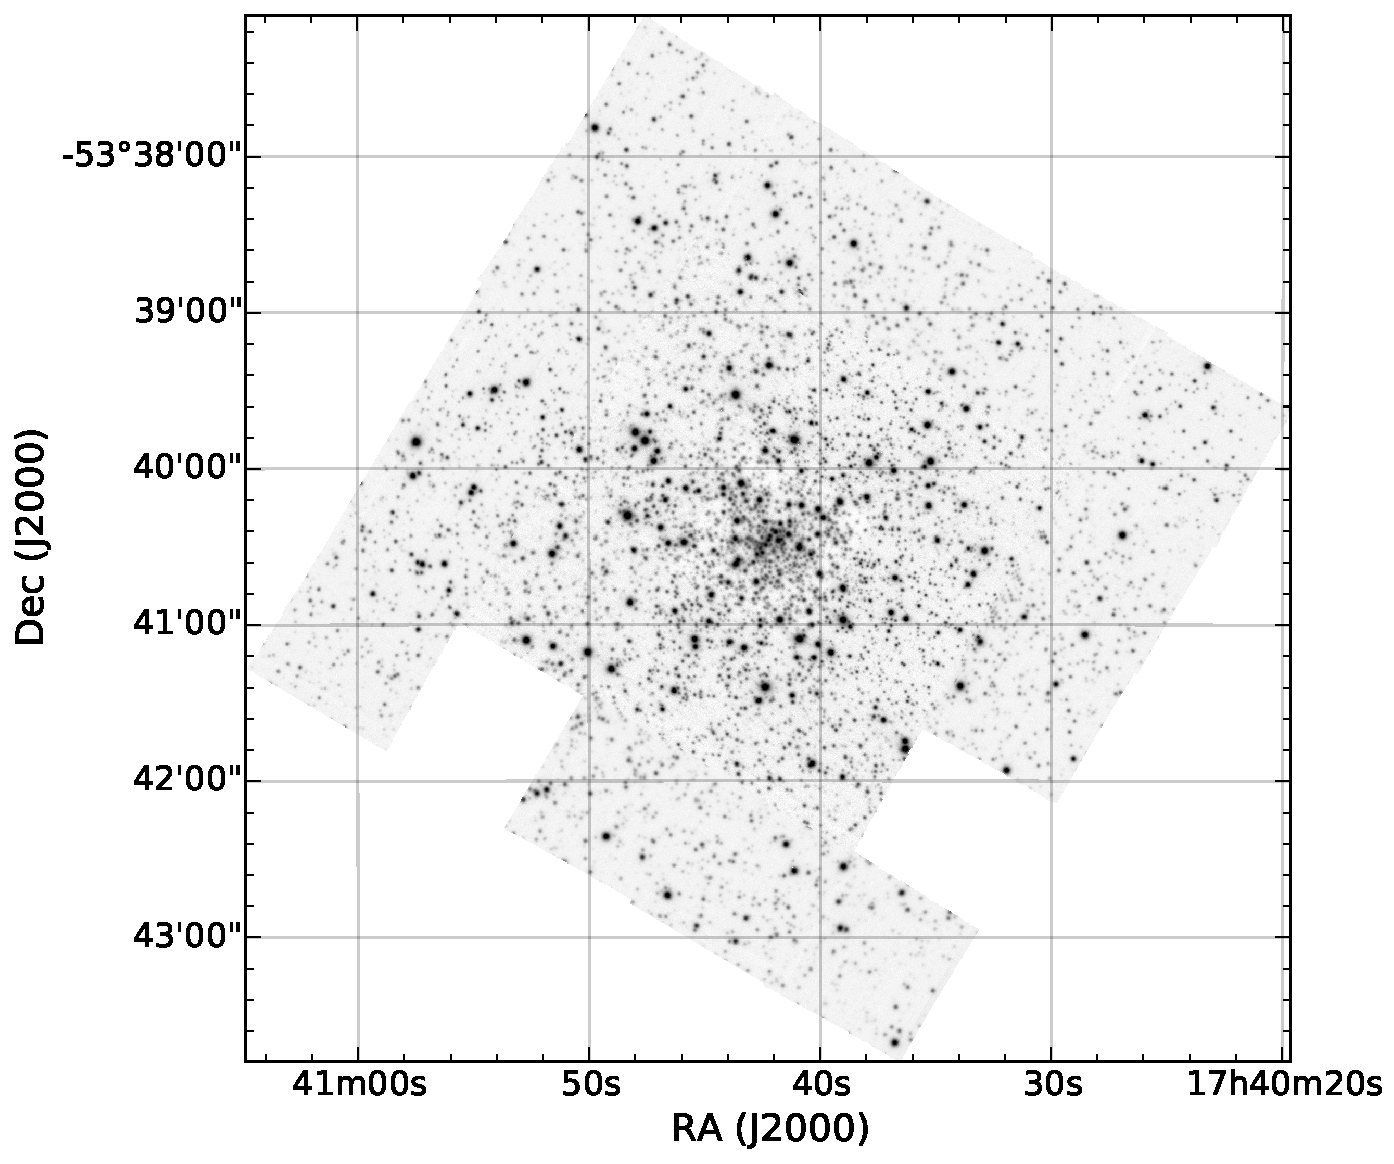
\includegraphics[scale=.6]{assets/images/mosaic.pdf}
\caption{bfagagaga}
\label{fig:clustermuse}
\end{figure}

\section{Processed and Raw data} 

The primary goal of the MUSE observation of NGC 6397 was to create the first comprehensive Hertzsprung-Russell diagram with a sample of over 12 000 spectra \citep{husser_muse_2016}. The large number of spectra obtained allow them to study the kinematics of the globular cluster with the goal to probe the presence of a central black hole in the cluster \citep{kamann_muse_2016}. This data is publicly available thought the \emph{MUSE Science Web Service}\footnote{\url{http://muse-vlt.eu/science/}}. The website contains advanced science products such as reduced datacubes, source catalogs and software tools. For NGC 6397 it can be found the release of the spectra of the globular cluster NGC 6397 as published in the studies mentioned above (\cite{husser_muse_2016} and \cite{kamann_muse_2016}). They provide all the obtained spectra with a signal-to-noise ratio of five or larger, i.e. 14271 spectra in total. For our goal to study the CVs in the globular clusters the data wasn't enough as it mainly covers the range from main sequence to the tip of the red giant branch\footnote{The red giant branch is }. Our approach in this project was to work with the raw science data. The science data can be obtained from the ESO  Science Archive Facility. As stated in the ESO Data Access Policy\footnote{\url{http://archive.eso.org/cms/eso-data-access-policy.html}} all science data is made publicly available through the science archive after the proprietary period (normally one year after the data have been made available to the principal investigator) and all calibration data are public immediately after the observations.  

\subsection{Data Reduction}

The data was reduced with version 1.2.1 of the MUSE Instrument Pipeline Recipes\footnote{The MUSE pipeline can be found at \url{http://www.eso.org/sci/software/pipelines/muse/}}\citep{weilbacher_design_2012}. The pipeline distribution kit includes several packages. The ones used for this work are the following:

\begin{itemize}
        \item The Common Pipeline Library version 6.6 \citep{mckay_common_2004}
        \item The ESO Recipe Execution Tool (EsoRex)\footnote{EsoRex is written by the CPL group (Pipeline System Department) European Southern Observatory \url{http://www.eso.org/sci/software/cpl/esorex.html}} version 3.12.
\end{itemize}

All the data reduction was done calling EsoRex to execute the MUSE DRS recipes from a bash (version 4.3.11) script\footnote{All the configuration files for each of the called MUSE recipes used, the bash scripts, useful python (Python 2.7.6) scripts and other text files relevant for the data reduction can be found at \url{https://github.com/manuelmarcano22/muse2016}} (alternative this can be done via the Python bindings \citep{streicher_python_2012}). We summarize the main steps to produce the fully reduced datacube from the raw science and calibration data download from the ESO Science Archive MUSE Query Form: 

\begin{enumerate}
        \item Calibration and pre-processing
                \begin{enumerate}[I]
        \item \textbf{Bias substraction}: Bias subtraction was done by combining 10 different bias images into one master bias file. Each bias is part of the calibration files taken by ESO every night.   
        \item \textbf{Flat-fielding}
        \item \textbf{Wavelenght calibration}: Detect arc emission lines and determine the wavelength solution for each slice.
        \item \textbf{Line Spread Function}
        \item \textbf{Geometrical calibration}
        \item \textbf{Illumination Correction}:
    \end{enumerate}
\item Post-processing
                \begin{enumerate}[I]
                        \item \textbf{Flux calibration}
                        \item \textbf{Sky substraction}
                        \item \textbf{Astrometry}
                        \item \textbf{Combination} K-means from 
                \end{enumerate}
\end{enumerate}


\subsection{Spectra extration and analysis}

Astropy, a community-developed core Python package for Astronomy \citep{astropy_collaboration_astropy:_2013}

IRAF (image reduction and analysis facility) \footnote{IRAF is distributed by the National Optical Astronomy Observatories, which are operated by the Association of Universities for Research in Astronomy, Inc., under cooperative agreement with the National Science Foundation} \citep{1986SPIE..627..733T},   


PyRAF\footnote{PyRAF is a product of the Space Telescope Science Institute, which is operated by AURA for NASA. \url{http://www.stsci.edu/institute/software_hardware/pyraf}}.



APLpy: This research made use of APLpy, an open-source plotting package for Python hosted at http://aplpy.github.com

scikit-learn \citep{scikit-learn}

\begin{comment}
Good data reduction steps in https://arxiv.org/pdf/1411.7667.pdf

version (1.2.1) designed by \citeauthor{weilbacher_design_2012} (see \cite{weilbacher_design_2012}) 

For the basic calibration we followed the standard procedure
to reduce MUSE data: combine 10 bias images to form a master
bias, combine 5 lamp-flat exposures, and use one exposure
of each arc lamp to derive the wavelength solution. 11 skyflats,
taken during the evening twilight preceding the science exposures,
were combined and used to create a 3D correction of the
illumination in the range λ = 5000 . . . 8000 Å2
.
The geometry of the instrument was derived f

. These calibrations were found
to be valid for the full period of the first commissioning run of
the instrument and were also shipped with the MUSE pipeline.

\end{comment}
